%!TEX root = ../Main.tex

\chapter{Vulkan Development Environment}
\label{cha:EnvSetup}
  \todo[inline]{Proper introduction to the chapter}

  % This chapter is a guide to setting up a Vulkan development environment in the context of \gls{ccpp} on a \gls{windows} operating system.

  % As can be expected, the steps required to setup a Vulkan environment depend on the development platform of choice.

  This chapter describes some practical aspects of Vulkan development and acts as a guide in setting up a Vulkan development environment.
  As can be expected, the steps required for such a setup depend on the kind of platform to be developed on.
  This chapter introduces the Vulkan Common Loader, which is used to interface with \glspl{icd} and Vulkan layers, the LunarG Vulkan \gls{sdk}, how to develop shaders for Vulkan applications, and discusses debugging and profiling capabilities.

  \section{Hardware Vendor Support}
  \label{sec:HardwareVendorSupport}
    Using and developing Vulkan applications requires support from the hardware.
    Information about Vulkan support for a particular piece of hardware can usually be found in the manual or on the hardware vendor website.
    There are also third-party resources that can be consulted to check whether a particular piece of hardware provides Vulkan support.
    The \textit{Vulkan Hardware Database}~\cite{vulkangpuinfo} is one such resource.
    This database even provides an overview of the supported hardware features and device extensions.

    In order to support Vulkan, hardware vendors have to provide driver implementations for the platform the user is targeting.
    These driver implementations are called \acrfullpl{icd}.
    How an \gls{icd} is chosen by the application is described in section~\ref{sec:VulkanLoader}.

    \todo[inline]{Check the following par.}

    At the time of writing, \gls{amd} and \gls{nvidia} are known to provide hardware and compatible drivers supporting Vulkan for use on \gls{windows}.
    In the early days of Vulkan, these companies only provided beta-quality \glspl{driver} but have released consumer-grade versions by now.
    \gls{intel} also provides beta-quality drivers for Windows but does not intend to release consumer-grade \glspl{driver} for the time being~\cite{intelvulkandriversonwindows}.

  \section{Vulkan Header}
  \label{sec:VulkanHeader}
    The Vulkan header file is generated from a more abstract representation called the Vulkan API Registry.
    The most recent version can be found in the Vulkan-Docs repository on GitHub, which can be found in the Khronos Vulkan Registry~\cite{vulkanregistry}.
    This repository contains the generated \gls{ccpp} header file.
    It also contains the file \lstinline{vk.xml} and a set of tools to generate the Vulkan header from it.

    \lstinputlisting[
      label=lst:VkFenceCreateInfo_vkxml,
      caption={The definition of \lstinline{VkFenceCreateInfo} as found in \lstinline{vk.xml}.},
      style=MyXML,
      float
    ]
    {Main/Listings/VkFenceCreateInfo_vkxml.xml}

    \lstinputlisting[
      label=lst:VkFenceCreateInfo,
      caption={The result of generating C bindings from listing~\ref{lst:VkFenceCreateInfo_vkxml}.},
      style=MyCppFloat,
      float
    ]
    {Main/Listings/VkFenceCreateInfo.txt}

    The \lstinline{vk.xml} essentially contains annotated C code with XML markup.
    The annotations also contain contextual information, something pure C code could not easily or conveniently provide in a standard way.
    Listing~\ref{lst:VkFenceCreateInfo_vkxml} shows the definition of a Vulkan structure as defined in the \lstinline{vk.xml} file.
    For this particular entry, the resulting Vulkan header file will contain the definition shown in listing~\ref{lst:VkFenceCreateInfo}.

    This additional layer of abstraction is useful to generate the Vulkan API in different ways.
    For example, when using \gls{cpp}, structures and functions may be reorganized into classes and methods instead, resulting in a code style that is more common in \gls{cpp}.
    It also makes it easier to generate native bindings for other programming languages, such as \gls{csharp} or \gls{python}.
    Line 10 of listing~\ref{lst:VkFenceCreateInfo_vkxml} shows the xml attribute \lstinline{optional="true"}.
    It basically states that it is allowed to pass a flags value of zero, i.e. no flags are set.
    Such an annotation would not be possible in regular C code.
    This is the main advantage of expressing the Vulkan API in this abstract format.


  \section{Vulkan Common Loader}
  \label{sec:VulkanLoader}
    \todo[inline]{How to handle overlapping topics discussed earlier, e.g. layers and extensions? Shorten in chapter 2 to minimize redundancy}

    \begin{figure}
      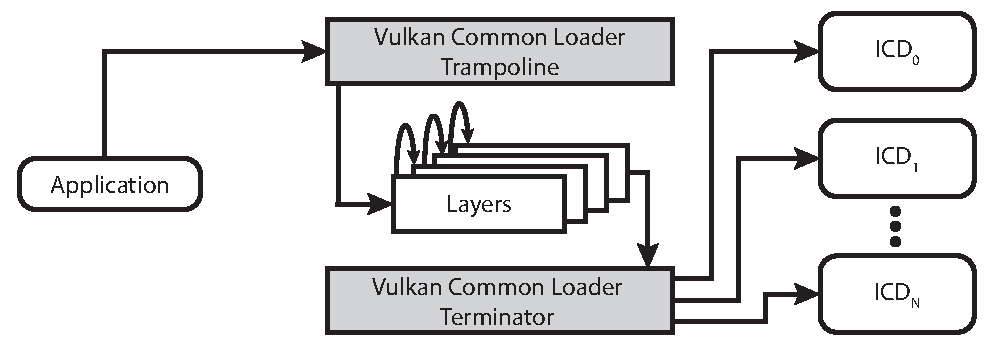
\includegraphics[width=\textwidth]{Main/Images/VulkanLoaderInstanceLayers}
      \centering
      \caption{Communication between the application and the \acrfullpl{icd} via the \gls{vkloader} when using instance-level API calls.}
      \label{fig:VulkanLoaderWithInstanceLayers}
    \end{figure}

    \begin{figure}
      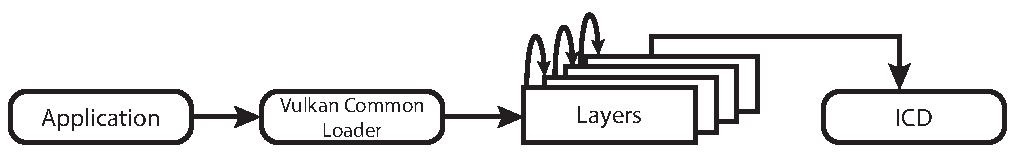
\includegraphics[width=\textwidth]{Main/Images/VulkanLoaderDeviceLayers}
      \centering
      \caption{Communication between the application and an \acrfull{icd} via the \gls{vkloader} when using device-level API calls.}
      \label{fig:VulkanLoaderWithDeviceLayers}
    \end{figure}

    The \gls{vkloader} is the interface between Vulkan applications and \glspl{icd}.
    It is an open source project mainly developed and maintained by the Khronos Group.
    It can be found in the Khronos Vulkan Registry~\cite{vulkanregistry}.
    It is written in \gls{c} and can be used by application developers either as a statically or dynamically linked library.
    It ensures that multiple \glspl{icd} can be installed on the same system without interfering with each other.
    It is also responsible for managing optional modules, called \textit{layers}.
    These layers are implemented as software libraries.
    There are explicit and implicit layers.
    Explicit layers can only be enabled when the Vulkan application requests these layers explicitly.
    \todo{Elaborate on controlling layer activation}This is done when creating a Vulkan instance or a Vulkan device.
    Implicit layers, on the other hand, are activated by default.

    \subsection{Interaction with an ICD}

    As explained in section~\ref{sec:WorkflowAndPatterns}, the first Vulkan object that has to be created by every application is the Vulkan instance.
    This instance can be used to query all layers that are available for that Vulkan instance.
    In this section, the process of loading Vulkan commands and interacting with the \gls{driver} and all layers in-between is looked at in more detail.

    \lstinputlisting[
      label=lst:VulkanFunctionLoading,
      caption={Pseudocode for loading different Vulkan functions using the common loader module on a Win32 platform.},
      style=MyCppFloat,
      float,
      emph={vkGetInstanceProcAddr, vkGetDeviceProcAddr}
    ]
    {Main/Listings/VulkanFunctionLoading.txt}

    \lstinputlisting[
      label=lst:VkInstanceCreateInfo,
      caption={Definition of the \lstinline{VkInstanceCreateInfo} structure.},
      style=MyCppFloat,
      float,
      emph={ppEnabledLayerNames, ppEnabledExtensionNames}
    ]
    {Main/Listings/VkInstanceCreateInfo.txt}

    \lstinputlisting[
      label=lst:VkDeviceCreateInfo,
      caption={Definition of the \lstinline{VkDeviceCreateInfo} structure.},
      style=MyCppFloat,
      float,
      emph={ppEnabledExtensionNames}
    ]
    {Main/Listings/VkDeviceCreateInfo.txt}

    In addition to what has been described so far, a layer is also able to provide several Vulkan \textit{extensions}.
    These extensions may define additional Vulkan commands that can be queried via the common loader using \lstinline{vkGetInstanceProcAddr} and \lstinline{vkGetDeviceProcAddr}, which are Vulkan commands to retrieve addresses of functions that are identified by their name.
    Usage of these Vulkan commands, in the context of a \gls{windows} operating system platform, is demonstrated in listing \ref{lst:VulkanFunctionLoading} as pseudocode.

    On the first line, the \gls{winapi} is used to load the \gls{vkloader}, simply called \lstinline{Loader} in the sample.
    On this platform, the \gls{vkloader} for Vulkan specification 1.0 and above is a \gls{dll} and is called \textit{vulkan-1.dll}.

    Continuing in the sample, the next step is to acquire the function \lstinline{vkGetInstanceProcAddr} from the Loader module.
    The \lstinline{vkGetInstanceProcAddr} function is used to load function addresses from the Loader module that are tied to a specific Vulkan instance.
    This Vulkan instance is passed to the \lstinline{vkGetInstanceProcAddr} function as the first argument.
    The second argument is the name of the function to load.

    On line 3 in the sample, \lstinline{NULL} is passed as the Vulkan instance.
    This is only allowed for a small set of functions that are not directly tied to a specific Vulkan instance.
    \lstinline{vkCreateInstance} is one such function, which is subsequently used to create a Vulkan instance on line 4.
    The first argument to \lstinline{vkCreateInstance} is an instance of the \lstinline{VkInstanceCreateInfo} structure.
    Among other things, this structure is used to enable a set of layers and extensions.
    The underlined elements in listing~\ref{lst:VkInstanceCreateInfo} show the relevant fields in order to enable the respective layers and extensions.

    In line 5 the address of the Vulkan command \lstinline{vkCreateDevice} is acquired.
    Instead of passing \lstinline{NULL}, this time the actual Vulkan instance is passed.
    This is done in order for the loader to know which active layers have to be notified about this call since they might have registered hooks to intercept the calls when creating a Vulkan device.

    In the next line, a Vulkan device is created using the previously fetched Vulkan command.
    During this call, all active and relevant layers, meaning all those layers that registered a hook for this case, are traversed and notified about this call.
    Similar to the process of creating a Vulkan instance, when creating a device, the application can request certain \textit{device extensions} to be activated.
    As can be seen in listing~\ref{lst:VkDeviceCreateInfo}, the process of requesting these extensions is the very similar to requesting instance-level extensions.

    Line 7 acquires the address to the Vulkan command called \lstinline{vkGetDeviceProcAddr} which is used to acquire function addresses from a specific \gls{icd}.
    This way, the Vulkan application can get the implementation of a command directly from the \gls{icd}.
    This alleviates the work required from the \gls{vkloader} as it does no longer have to look up the correct \gls{icd} for the context of the current call.

    Lines 8 and 9 are just examples of how a device-specific command is queried and executed.
    Just like before, the \gls{vkloader} will make sure all relevant layers are notifed about this call, even though this time it is a device-specific call as opposed to an instance-specific call.

    In performance-critical applications care must be taken when activating layers in a production scenario.
    Because every layer is called in order, every layer introduces additional overhead per \gls{api} call.
    Validation layers, for example, are typically not desired in a production scenario.
    At the time of writing there is no standard way to get \gls{icd} modules using the \gls{vkloader}.
    However, because of the \gls{vkloader} being open-source software, a developer is able to extract the relevant loader logic, customizing it to their specific needs.
    This should only be done if absolutely necessary because it requires the developer to maintain their port of the \gls{vkloader} in case future revisions of the original \gls{vkloader} change internal behavior or layer and extension conventions crucial for proper execution of the application.
    Otherwise the developer risks that their application stops working because of incompatibilities.
    After all, internals or conventions introduced by the original \gls{vkloader} are not standardized or specified by Vulkan.

    \todo[inline]{Device extensions are for vendor-specific extensions, such as NV\_glsl that support loading glsl shader code. For more on shaders see sec:EnvShaders.}

    \todo[inline]{Layers are discovered by the loader via the registry on Windows and in special directories on Unix based platforms. Files discovered there are always in JSON format and provide information about the library location and more. \lstinline{HKEY_LOCAL_MACHINE\\SOFTWARE\\Khronos\\Vulkan}}

    \todo[inline]{Dissect an example JSON file and explain the parts here?}

    \todo[inline]{Mention that the order in which layers are activated matters?}


  \section{LunarG Vulkan SDK}
  \label{sec:LunarGSDK}
    The LunarG Vulkan \gls{sdk}~\cite{lunargvulkansdk} is a \acrlong{sdk} developed by LunarG.
    LunarG is a software company that develops tools and infrastructure for Vulkan development.
    The company itself is sponsored by Valve Corporation.
    The first version of the LunarG \gls{sdk} was released at the same time as version 1.0 of the Vulkan specification.

    Developing a Vulkan application does not require the LunarG \gls{sdk} to be installed.
    For that, only the Vulkan header and common loader are required.
    However, the LunarG \gls{sdk} includes these two components and a number of additional components.
    These components are meant to help making it easier to develop Vulkan applications.
    Aside from the Vulkan header and the common loader, the \gls{sdk} also includes several Vulkan layers, debugging tools, tools that aid in creating shader modules compatible with Vulkan, the Vulkan API documentation, and a range of Vulkan samples and demos as well as a sample-driven tutorial.

    \todo[inline]{Introduce the \lstinline{vulkaninfo} command.}


  \section{Shaders}
  \label{sec:EnvShaders}
    As mentioned in section~\ref{sec:Pipelines}, Vulkan expects shaders to be in \gls{spirv} format.
    \gls{spirv} is a binary format and is not meant to be human-reabable.
    Instead of writing shaders directly in \gls{spirv} format, they are usually written in \gls{glsl} and converted to \gls{spirv} in a subsequent step.
    This tool is called \textit{glslangValidator}~\cite{glslangrepo} and is a command-line based tool that is able to validate \gls{glsl} code and to convert it into other representations.
    \todo{Describe what exactly is required. layout=N, binding=N, set=N, \#extensionm, ...}It requires the \gls{glsl} source code to be written in a specific way in order to be converted to \gls{spirv}.

    \todo[inline]{explain that shaders can be converted in different shader stages, e.g. vertex-, fragment-stage, hence the file endings and filenames}

    \lstinputlisting[
      label=lst:glslangcmd,
      caption={Sample usage of the program called \lstinline{glslangValidator}.},
      style=MyCppFloat,
      float
    ]
    {Main/Listings/glslangValidator.txt}

    Listing \ref{lst:glslangcmd} shows how to convert two shader programs, provided in \gls{glsl} format, to \gls{spirv} using Glslang.
    The \lstinline{-V} switch tells Glslang to convert to Vulkan-compatible \gls{spirv} format.
    The \lstinline{-o} switch is used to control how the output file is named.
    In the first line, the input is the file called \lstinline{Shader.vert} and the output is a file called \lstinline{Vertex.spv}, which will be in \gls{spirv} format.
    The second line does the same transformation for the input file \lstinline{Shader.frag} and the output file \lstinline{Fragment.spv}.

    Another approach is to use a custom-made front-end that would be convertible to \gls{spirv}.
    This might be the favorable approach for many graphics or game engines since these technologies \todo{Do I need references here?}usually have their own abstract representation of shader functionality.
    Being able to directly translate to \gls{spirv} removes the need to translate into some human-readable form first, such as \gls{glsl}, as was the case with \gls{opengl}.


  \section{Debugging and Profiling}
  \label{sec:DebuggingAndProfiling}
    The layered architecture of Vulkan makes it straight-forward for tool developers to provide debugging and profiling capabilities that integrate seamlessly with existing Vulkan applications.
    These tools usually just offer one or more layers, and possibly some extensions, that are either implicitly or explicitly activated.

    The LunarG Vulkan \gls{sdk} comes with a variety of layers, many of which are debugging layers.
    It also provides a layer which combines all debugging layers in one layer in an optimal order called \lstinline{standard_validation}\footnote{Full name: \lstinline{VK_LAYER_LUNARG_standard_validation}}.
    All these debugging layers, including the standard validation layer, are explicit layers that have to be activated when creating a Vulkan instance.
    Layers have been described in section~\ref{sec:LayersAndExtensions} and the careful reader might have noticed that layers do not get back in touch with the Vulkan application directly.
    \todo{Find out where this extension is coming from? i.e. from which layer. Seems like all layers provide it?!}For this purpose the \lstinline{VK_EXT_debug_report} extension is used.
    This extension provides additional Vulkan commands that can be used to supply a callback that will be triggered whenever a layer, that supports the debugging interface, needs to communicate back to the Vulkan application.
    For example, when a validation layer detects erroneous input, it will invoke the supplied debug callback and inform the application of invalid behavior.

    Another tool for debugging, that is also supplied with the LunarG Vulkan \gls{sdk}, is RenderDoc~\cite{renderdoc}.
    RenderDoc is a graphics debugging tool that allows the developer to inspect pipeline states at each \gls{api} invocation.
    RenderDoc has provided \gls{d3d} and \gls{opengl} support for quite some time already but also provides Vulkan support since the release of Vulkan 1.0.
    When RenderDoc is installed, it also installs the implicit layer called \lstinline{VK_LAYER_RENDERDOC_Capture}.
    This means that any Vulkan-enabled application can be debugged using RenderDoc.
    This layer is used to capture \gls{api} calls and track state in that way.
    In order for RenderDoc to work, it has to be hooked up with the Vulkan application that is to be inspected.
    Once hooked up, RenderDoc is rendering a small amount of statistics, such as current framerate, in the upper left corner of the applications window.
    It also shows which button to press to instruct RenderDoc to \todo{elaborate on the term "capture" and what it actually does}capture a frame.
    Once a frame was captured it can be inspected inside of the RenderDoc UI.
    This captured frame contains, among other things, the state of the frame buffers but also records \gls{api} calls, shows their \gls{cpu} execution time, shows bound textures for active shaders, and more.

    Once a Vulkan application is running correctly, the developer might also be interested in whether it runs \textit{efficiently}.
    This is especially important for many real-time applications such as video games.
    Due to the young age of Vulkan, there are not many profiling tools specifically tailored towards Vulkan applications.
    There are some tools that can aid in this regard, though.
    The LunarG SDK, as described in section~\ref{sec:LunarGSDK}, offers API tracing and playback tools.
    These tools effectively record which commands are performed by an application, measuring the execution time of individual commands.
    This can help in tracking down bottlenecks observed on the host-side.
    The RenderDoc Graphics Debugging Tool~\cite{renderdoc} also has the capability of tracking API calls.
    However, tools of this kind are not capable of capturing how the GPU behaves for a given Vulkan application.
    At the time of writing, no Vulkan-specific GPU profiling tool is available as known to the author.

    % For measuring \gls{gpu} behavior on a more general scale, other tools can be used.
    % One such tool is \gls{nvidia} FCAT~\cite{nvidiafcat}.
    % This tool requires a special piece of hardware, called a \textit{capture card}, that captures the output of a graphics card and displays analysis results directly on the attached computer display.
    % Thus, it does not rely on application-specific, internal measurements.
    % Usage of this tool is not wide-spread but
    % Usage of this tool is note wide-spread, but at least some computer magazines use it for benchmarking when comparing different models of graphics and compute harcware~\cite{eurogamer2016:doomvulkan}\todo{citations! At least 2.}.

    The Vulkan \gls{api} itself also provides so-called \textit{timestamp queries}.
    These queries can be used to insert special query commands into a command buffer to write a timestamp value into a \textit{query pool}.
    The results recorded in the query pool can then be read from the host at certain times.
    \todo{Is this comprehensive enough?}This enables application developers to implement their own internal \acrshort{gpu} profiling system by taking time samples at application-defined points within command buffers.
    See section~16.5 of the Vulkan specification~\cite{vkspec} for details.

    \todo[inline]{Omit the following paragraph?}
    % \todo{Better phrasing? Make it more formal.}Vulkan has only been around for a short while now.
    Vulkan is still relatively new technology.
    Existing tools for other graphics \glspl{api} will most likely be extended to also support Vulkan.
    It is also possible that new tools dedicated to Vulkan may be developed by \glspl{ihv}.
